\documentclass[letterpaper,12pt]{article}

\usepackage{listings}
\usepackage{hyperref}
\usepackage{graphicx}

\lstdefinestyle{code}{
	basicstyle=\ttfamily\small
}

\lstset{style=code}

\graphicspath{ {./figures/} }

\begin{document}
\title{A Curious Case of Complex Codomain Coloring}
\author{Jake Looney\\ Undergrad at the University of Tennessee Knoxville}
\date{January 2022}
\maketitle

\pagenumbering{roman}
\tableofcontents
\newpage
\pagenumbering{arabic}

\section{Motivation}
I ain't gonna lie, I was really high when I wrote the code for this and was trying to just make a domain coloring grapher.
I had seen a couple of pictures on Wikipedia using domain coloring and saw the term so I decided to just have a go at it.
I was thinking that "domain coloring" would make sense to color the domain and then apply the function.
Of course, normal domain coloring works the other way, where you apply the function then color based on where the points land.
So, what resulted is the other direction of the usual way to do this: points are colored based on their preimage.
This requires some working around in order to work with general functions.
There's not many reasons to do this: it goes against the standard, its computationally intensive, slow as shit, blocky, imprecise, and only shows one point in the preimage per point in the image.
However, despite this, I did discover something pretty interesting while shoving fun functions into it. But first, an explanation of the code.

\section{Code explanation}
There is an attached GitHub repository containing the code. You can view it here: \url{https://github.com/6a6c/jraph} \\

The function \verb|createPicture| takes a map of pixel indices and complex points to output a bitmap image.
It mainily utiliizes a bitmap implementation I stole from class, but importantly it colors points in the image based on their argument and magnitude:
\begin{lstlisting}[language=c++]
    z = fit->second;
    mag = abs(z);
    ar = arg(z);

    pixarray[fit->first].red = min(5*mag, 255.0);
    pixarray[fit->first].blue = min(40*ar, 255.0);
    pixarray[fit->first].green = min(100*mag, 255.0);
\end{lstlisting}
This can be changed in order to alter the colorscheme, but I have no idea what the hell LAB color is so I will have to come back to it.\\

There are three main functions that are used to create these graphs. The function \verb|makeFunction| creaates a multimap of doubles corresponding to output magnitudes and a pair of complex points corresponding to input and output points of a function. To do this, it applies a function to a region of complex points and adds them to the multimap:
\begin{lstlisting}[language=c++]
for( i = -1 * pts; i < pts; i++){
  for( j = -1 * pts; j < pts; j++){

    z = complex<double>(aCoeff * i * i * i, aCoeff * j * j * j);
    output = complex<double>(0,0);
    k=0;
    while(k < mandoIters && abs(output) < 2){
      output = pow(output, 2) + z;
      k++;
    }
    if(abs(output) > 2) output = complex<double>(INFINITY, 0);

    //output = sin(z);
    //output = (((z * z) + complex<double>(-1,0)) 
    //		* pow((z + complex<double>(-2, -1)), 2))
    //           /(z*z + complex<double>(2,2));
    //output = ((z * z * z) + complex<double>(-1, 0));
    //output = z;

    function->insert(make_pair(abs(output), make_pair(output, z)));

  }
}
\end{lstlisting}
The points selected to be input points for the function are scaled based on a cubic function.
This means that there are more points around 0 (the interesting parts) and less points further out.
The coefficient on the cubic as well as the number of points can be changed.
Currently, the function being applied in this code is the Mandlebrot function, with the ability to change the number of iterations (see section 4).
However, other example functions are commented out, and the comments can be changed to change the function applied. \\

The function \verb|makeMap| is used to create the maps that are passed to \verb|createPicture|.
To do this, it is passed a multimap created by \verb|makeFunction| as well as the boundaries of a region on the complex plane.
It inserts points into the map based on their preimage by passing points to \verb|preImage| based on the region.
\begin{lstlisting}[language=c++]
for(i = 0; i < w * h; i++){
  complex<double> z(realLeft + ((i\%w) * ((realRight - realLeft)/w)),
			imagTop - ((i/w) * ((imagTop - imagBot)/h)));

  complex<double> pre = preImage(z, function);

  ret->insert(make_pair(i, pre));

}
\end{lstlisting}
\verb|preImage| works by first isolating a range of the function multimap with magnitudes within a certain ammount of the image point z.
Then, it iterates through this range and finds the point with the least distance from z.
The input point that corresponds to this output point (that is, second part of the pair in the multimap).

\begin{lstlisting}[language=c++]
double mag = abs(z);
double d1, d2, best;
map< double, pair< complex<double>, complex<double> >
    >::const_iterator low, high, fit, bit;
size_t i = 0;

low = func->lower_bound(mag-(ep * mag));
high = func->upper_bound(mag+(ep * mag));

bit = low;
best = 100000;
for(fit = low; fit != high; fit++){
  d1 = sqrt( pow(z.real() - fit->second.first.real(), 2) +
       pow(z.imag() - fit->second.first.imag(), 2) );

  if(d1 < best) {
    best = d1;
    bit = fit;
  }

}

return bit->second.second;

\end{lstlisting}

The result, after calling \verb|preImage| on all the points for the picture, is a preimage point for each point in the codomain. \\ \\

\section{That's cool, but what do the pictures look like?}

For reference, it's important to see what the unaltered complex plane (that is to say, the domain) looks like:

\begin{figure}[h]
	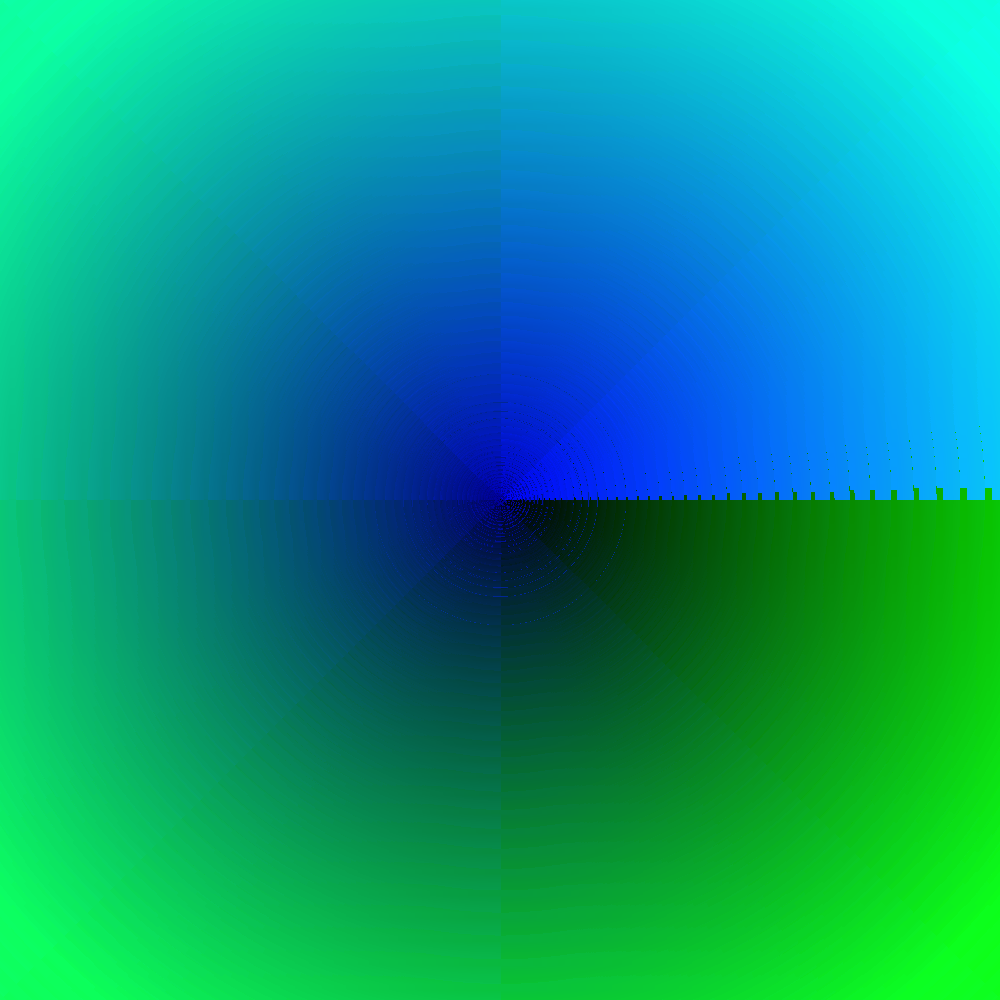
\includegraphics[width=8cm]{f(z)=z}
	\centering
	\caption{f(z) = z}
	\centering
\end{figure}

This image was obtained by using f(z) = z as the function through the codomain grapher.
This can be thought of as the domain for other functions, the complex plane before a function is applied to it.

\end{document}
